\documentclass[conference]{IEEEtran}

% ============================================================
% TriNetra: IEEE Conference Research Paper
% ============================================================
% IMPORTANT:
% 1. This manuscript is grounded in the supplied TriNetra copyright,
%    implementation/status documents, and supplied RGB-T literature.
% 2. Do NOT replace placeholders with invented experimental results.
% 3. The current as-built status supports Phase 1--3 and TRC evaluation.
%    TRC-gated YOLOv8 fusion and downstream tracking/threat modules are
%    described as the planned research pipeline unless independently
%    verified by your final experiments.
% ============================================================

\usepackage{cite}
\usepackage{amsmath,amssymb,amsfonts}
\usepackage{algorithm}
\usepackage{algpseudocode}
\usepackage{graphicx}
\usepackage{booktabs}
\usepackage{multirow}
\usepackage{array}
\usepackage{url}
\usepackage{xcolor}
\usepackage{tikz}
\usepackage{pgfplots}
\usepackage{balance}
\usepackage{microtype}
\usepackage{enumitem}
\usepackage{caption}
\usepackage{subcaption}
\usepackage{adjustbox}
\usepackage{tabularx}
\usepackage{makecell}

\usetikzlibrary{arrows.meta,positioning,fit,calc,shapes.geometric,shapes.misc,backgrounds}

\pgfplotsset{compat=1.18}
\captionsetup{font=footnotesize}
\setlist{nosep,leftmargin=*}

% ---------- Project colours ----------
\definecolor{trcPurple}{RGB}{92,62,140}
\definecolor{rgbBlue}{RGB}{40,100,180}
\definecolor{thermalOrange}{RGB}{220,120,35}
\definecolor{detectGreen}{RGB}{45,125,75}
\definecolor{threatRed}{RGB}{175,55,55}
\definecolor{lightGray}{RGB}{245,245,245}

% ---------- Placeholder figure command ----------
\newcommand{\figplaceholder}[3]{%
\begin{figure}[!t]
\centering
\fbox{%
\begin{minipage}[c][#2][c]{0.94\columnwidth}
\centering
\textbf{FIGURE PLACEHOLDER}\\[4pt]
#1\\[4pt]
\textit{Replace this box with the final exported figure.}
\end{minipage}}
\caption{#3}
\label{fig:#1}
\end{figure}}

\begin{document}

% ============================================================
% TITLE / AUTHORS
% ============================================================

\title{TriNetra: Real-Time RGB-T Threat Intelligence}

\author{
\IEEEauthorblockN{Dr Yogita Bhise, Aditya Ahirrao, Disha Kapse, Sadique Khatib, Vedant Sonawane}
\IEEEauthorblockA{
K. K. Wagh Institute of Engineering Education \& Research\\
Nashik, Maharashtra, India\\
}
}

\maketitle

% ============================================================
% ABSTRACT
% ============================================================


\begin{abstract}

RGB-thermal (RGB-T) perception combines complementary visible-spectrum
and thermal information and is particularly attractive for surveillance
under low illumination and adverse visual conditions. However, the
usefulness of either modality can vary with scene quality, sensor
degradation, blur, saturation, low contrast, and cross-modal
misalignment. Conventional fusion mechanisms may therefore propagate
unreliable information instead of suppressing it.

This paper proposes \textit{TriNetra}, a reliability-aware RGB-T
surveillance framework centered on the TriNetra Reliability Coefficient
(TRC). The primary research hypothesis is that explicitly estimating
the reliability of the thermal modality before RGB-T fusion can improve
the robustness of multimodal object detection compared with fixed-weight
fusion and single-modality processing, particularly under degraded
thermal conditions. TRC combines five interpretable cues: histogram
entropy-based contrast, Laplacian-variance gradient strength,
saturation/clipped-pixel ratio, normalized mutual information between
RGB and thermal observations, and alignment quality.

The current implementation provides RGB-T synchronization,
preprocessing, alignment handling, TRC computation, validation
analysis, and controlled thermal-degradation testing. On the supplied
80-frame validation subset, TRC has a mean of 0.758 with a standard
deviation of 0.024 and no sample below the configured 0.30 threshold.
Under controlled degradation, representative TRC values decrease from
clean thermal input to blur, saturation, and flat-response conditions.
These observations provide preliminary evidence consistent with the
hypothesis that TRC can act as an interpretable reliability control
signal.

A first working implementation of the TRC-gated fusion detector has
since been trained and evaluated end-to-end on real paired RGB-T data:
a preliminary Stage-1 run over 300 of the 9{,}903 available training
images (4 of a planned 20 epochs, CPU-only, batch size 4) was
evaluated on the complete, official LLVIP test split of 3{,}463 images
and reached mAP@0.50\,=\,0.770 and mAP@0.50:0.95\,=\,0.472, with
training loss falling every epoch. This establishes that the
architecture trains stably and generalizes to held-out data; it is an
absolute-performance measurement of TriNetra-v1 rather than a
comparative test of H1, since the single-modality and fixed-fusion
baselines required to isolate the effect of TRC gating have not yet
been run under an identical protocol. The paper defines the proposed
fusion architecture, research hypotheses, baseline comparisons,
ablation strategy, and evaluation protocol needed to complete that
comparison.

\end{abstract}


\begin{IEEEkeywords}
RGB-T object detection, multispectral surveillance, thermal reliability, adaptive fusion, modality failure, YOLOv8, threat intelligence, multimodal perception.
\end{IEEEkeywords}

% ============================================================
% I. INTRODUCTION
% ============================================================

\section{Introduction}

Reliable visual perception is a fundamental requirement for surveillance systems deployed in environments where illumination, atmospheric conditions, or sensor quality cannot be guaranteed. Conventional RGB cameras provide rich colour, texture, and contextual information, but their effectiveness can decrease substantially in darkness, glare, fog, smoke, rain, and low-contrast scenes. Thermal infrared sensors offer complementary information because their measurements are less dependent on visible illumination; however, thermal imagery generally provides less colour and texture information and can itself be affected by blur, saturation, weak thermal contrast, sensor interference, and registration errors. The complementary nature of visible and thermal sensing has consequently motivated extensive research in RGB-T image analysis, including fusion, pedestrian detection, object detection, tracking, and related tasks \cite{songSurvey}.

Recent RGB-T object detectors increasingly use dual-stream networks and feature-level fusion. TFDet, for example, addresses noisy fused feature maps through target-aware fusion and feature refinement, demonstrating the importance of suppressing background and false-positive features \cite{tfdet}. Quality-aware decision fusion has also been investigated through evidential deep learning and Dempster--Shafer theory to explicitly handle uncertainty and modality failure \cite{qdfm}. More recent approaches such as DENet use diffusion-based feature reconstruction, redundant-information suppression, and illumination-aware weighting to mitigate modality failure \cite{denet}. EEF further investigates energy-based feature enhancement and adaptive feedback for RGB-T feature fusion \cite{eef}. GEM-YOLO demonstrates that gated multimodal fusion can improve real-time RGB-T detection while controlling computational cost \cite{gemyolo}. These studies collectively indicate that multimodal detection performance depends not only on the availability of two sensors, but also on how their information is weighted and combined.

The central observation motivating TriNetra is that \emph{modality availability does not imply modality reliability}. A thermal frame may be present but provide poor information for a particular scene. Similarly, a visible frame may be severely degraded while its paired thermal image remains useful. A fusion mechanism that treats both streams identically can therefore introduce unreliable information into the fused representation. This issue is closely related to the broader multimodal fusion problem, in which complementary, redundant, and unreliable information must be integrated without allowing one source to dominate incorrectly \cite{deepFusion}.

TriNetra addresses this problem by introducing an explicit, interpretable thermal reliability signal before fusion. The proposed TriNetra Reliability Coefficient (TRC) aggregates five low-cost image-quality and cross-modal cues into a scalar in $[0,1]$. The score is subsequently used to determine the relative contribution of the thermal and RGB streams. The current implementation uses a scalar frame-level TRC, while a spatial reliability map is retained as an extension for future region-adaptive fusion. The project implementation documents specify a pipeline consisting of RGB-T synchronization, preprocessing, TRC computation, TRC-gated fusion, YOLO-based detection, tracking, behaviour analysis, threat reasoning, and explainable alert generation.

The contribution of this work is therefore not a claim that RGB-T fusion itself is novel, but a surveillance-oriented framework that places an interpretable, image-quality-driven reliability estimate between preprocessing and cross-modal fusion. The principal contributions are:

\begin{enumerate}
    \item An interpretable thermal reliability coefficient, TRC, computed from five normalized quality cues.
    \item A reliability-aware RGB-T fusion formulation in which the thermal contribution is controlled by TRC.
    \item A reproducible stress-test protocol for evaluating whether TRC decreases under controlled thermal degradation.
    \item A modular surveillance architecture connecting multimodal perception with detection, tracking, threat reasoning, and explainable alerts.
    \item A controlled ablation protocol comparing RGB-only, thermal-only, fixed RGB-T, TRC-gated RGB-T, and future learned-weight variants.
\end{enumerate}

\subsection{Research Hypotheses}

The primary hypothesis investigated in this work is:

\begin{quote}
\textbf{H1:} Reliability-aware RGB-T fusion using the TriNetra
Reliability Coefficient will provide more robust object detection than
single-modality processing and fixed-weight RGB-T fusion, particularly
when one modality is degraded.
\end{quote}

A secondary hypothesis is:

\begin{quote}
\textbf{H2:} TRC will decrease systematically as thermal-image quality
degrades, making it suitable as an interpretable control signal for
adaptive multimodal fusion.
\end{quote}

The current validation and stress-test experiments provide preliminary
evidence relevant to H2. A first end-to-end detection result is also
now available for TriNetra-v1 (Section~\ref{sec:results}), but H1
remains a testable research hypothesis: it is a \emph{comparative}
claim against single-modality and fixed-fusion baselines, and those
baselines have not yet been trained under the identical protocol
required to isolate the effect of TRC gating from the effect of
training data volume, epochs, or hardware.

The paper deliberately distinguishes the \emph{implemented and experimentally verified} TRC pipeline, and the preliminary TriNetra-v1 detection result, from downstream modules that remain subject to final end-to-end validation. This distinction is necessary to avoid reporting unverified detection or threat-assessment performance.

% ============================================================
% II. RELATED WORK
% ============================================================

\section{Related Work}

\subsection{RGB-T Image Analysis}

RGB-T analysis exploits complementary visible and thermal measurements and has been investigated extensively for detection, segmentation, fusion, tracking, and surveillance applications \cite{songSurvey}. The broad literature includes image fusion, salient object detection, semantic segmentation, pedestrian detection, tracking, and person re-identification \cite{songSurvey}. From a system perspective, multimodal fusion can be viewed at different stages of the processing pipeline, including input-level, feature-level, and decision-level integration. Modern multimodal learning further introduces attention, encoder-decoder, graph, generative, and constraint-based mechanisms \cite{deepFusion}.

For surveillance applications, the main advantage of RGB-T sensing is that the modalities exhibit different failure characteristics. RGB is typically rich in texture and colour but strongly dependent on visible illumination. Thermal sensing can preserve object signatures when illumination is poor, but may lose fine texture or become unreliable under sensor-specific degradations. This complementarity makes reliability-aware fusion an important design consideration.

\subsection{Adaptive and Target-Aware Fusion}

TFDet proposes a target-aware fusion strategy for RGB-T pedestrian detection. Its fusion-refinement design examines parallel and cross-channel similarities and uses a segmentation branch to separate pedestrian-related features from background features \cite{tfdet}. The reported results on KAIST, LLVIP, FLIR, and M3FD demonstrate the value of suppressing irrelevant fused features.

GEM-YOLO introduces an adaptive multimodal gated fusion mechanism together with lightweight architectural components for real-time RGB-T detection \cite{gemyolo}. The work is especially relevant to TriNetra because both approaches recognize that fixed or insufficiently adaptive fusion can be problematic. TriNetra differs in that the gating signal is explicitly tied to a hand-designed, interpretable thermal reliability score rather than being learned entirely inside the detector.

EEF introduces energy-score-guided feature enhancement, efficient cross-modal fusion, and adaptive feedback to improve modality representation \cite{eef}. This provides another example of using an explicit signal to influence multimodal feature processing. TriNetra instead emphasizes a low-cost quality signal that can be inspected independently of detector confidence.

\subsection{Modality Failure and Quality-Aware Decision Making}

Wang \emph{et al.} specifically investigate RGB-T detection under failure scenarios and propose DENet, which combines diffusion-based information reconstruction, redundant-information suppression, and a kernel-similarity-aware illumination module for dynamic modality weighting \cite{denet}. Their work directly motivates the need to evaluate multimodal systems under nonroutine conditions rather than only on clean benchmark data.

Yu \emph{et al.} propose quality-aware decision fusion using evidential deep learning and Dempster--Shafer theory \cite{qdfm}. Their approach expresses uncertainty at the decision level and reports improved performance under sensor interference and failure conditions. TriNetra shares the quality-awareness objective but operates earlier in the pipeline, estimating thermal reliability before feature fusion.

\subsection{Research Gap}

The supplied literature suggests three recurring directions: adaptive fusion, explicit treatment of modality failure, and robust decision making. However, the TriNetra design targets a different combination of properties. It seeks a \emph{simple, interpretable, detector-independent reliability signal} that can be computed before fusion and used to modulate the thermal contribution. The intended framework therefore provides:

\begin{itemize}
    \item an explicit numerical reliability signal;
    \item interpretable components that can be inspected individually;
    \item a direct connection between reliability and fusion weights;
    \item a degradation stress test independent of detector training;
    \item a modular interface that can be connected to different detectors.
\end{itemize}

This positioning is complementary to learned attention and decision-fusion approaches rather than a replacement for them.

% ============================================================
% III. SYSTEM OVERVIEW
% ============================================================

\section{TriNetra System Architecture}

The TriNetra framework is organized as a modular pipeline. The project documentation describes the intended sequence as dual-sensor acquisition, synchronization and preprocessing, TRC computation, reliability-aware fusion, YOLO detection, tracking and behaviour analysis, threat reasoning, and explainable alert generation. The current as-built implementation has completed the project scaffold, paired LLVIP data pipeline, and the alignment, denoising, normalization, and TRC stages. TRC-gated YOLOv8 fusion is the next major experimental stage.

\begin{figure*}[!t]
\centering
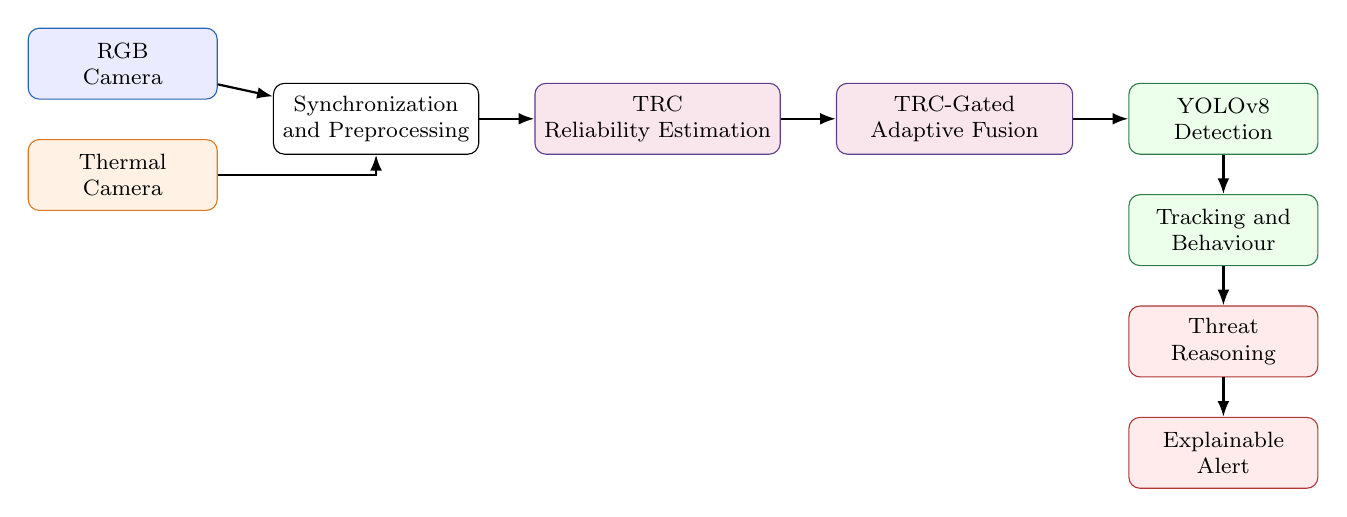
\begin{tikzpicture}[
node distance=5mm and 7mm,
block/.style={draw, rounded corners, align=center, minimum height=9mm, minimum width=24mm, font=\footnotesize},
rgb/.style={block, fill=blue!8, draw=rgbBlue},
thermal/.style={block, fill=orange!10, draw=thermalOrange},
fusion/.style={block, fill=purple!10, draw=trcPurple, minimum width=30mm},
greenblock/.style={block, fill=green!8, draw=detectGreen},
redblock/.style={block, fill=red!8, draw=threatRed},
arrow/.style={-{Latex[length=2mm]}, thick}
]
\node[rgb] (rgb) {RGB\\Camera};
\node[thermal, below=of rgb] (ir) {Thermal\\Camera};

\node[block, right=of rgb, yshift=-7mm] (prep) {Synchronization\\and Preprocessing};
\draw[arrow] (rgb) -- (prep);
\draw[arrow] (ir) -| (prep);

\node[fusion, right=of prep] (trc) {TRC\\Reliability Estimation};
\draw[arrow] (prep) -- (trc);

\node[fusion, right=of trc] (af) {TRC-Gated\\Adaptive Fusion};
\draw[arrow] (trc) -- (af);

\node[greenblock, right=of af] (det) {YOLOv8\\Detection};
\draw[arrow] (af) -- (det);

\node[greenblock, below=of det] (trk) {Tracking and\\Behaviour};
\draw[arrow] (det) -- (trk);

\node[redblock, below=of trk] (threat) {Threat\\Reasoning};
\draw[arrow] (trk) -- (threat);

\node[redblock, below=of threat] (alert) {Explainable\\Alert};
\draw[arrow] (threat) -- (alert);
\end{tikzpicture}
\caption{TriNetra end-to-end surveillance architecture. The solid blocks from sensing through TRC represent the implemented Phase 1--3 pipeline; downstream fusion, detection, tracking, threat reasoning, and alert modules form the intended end-to-end research pipeline and must be supported by final experiments before performance claims are made.}
\label{fig:architecture}
\end{figure*}

\subsection{Design Principle}

Let $I_R$ denote the visible image and $I_T$ the paired thermal image. The central design principle is:

\begin{equation}
R_T = f(I_R,I_T) \in [0,1],
\label{eq:trc_general}
\end{equation}

where $R_T$ is the thermal reliability estimate. A high value indicates that the thermal stream contains useful information for the current paired observation, while a low value indicates that its contribution should be reduced.

The implementation documentation specifies that LLVIP is treated as pre-aligned and that a pass-through identity transformation is used for the dataset. For general cases, homography estimation can use ORB/SIFT feature matching and RANSAC.

% ============================================================
% IV. TRC
% ============================================================

\section{TriNetra Reliability Coefficient}

\subsection{TRC Design}

The TRC is an unsupervised scalar reliability measure in $[0,1]$. It combines five cues:

\begin{enumerate}
    \item thermal contrast/information content;
    \item gradient or edge strength;
    \item saturation or clipped-pixel ratio;
    \item RGB--thermal mutual information;
    \item spatial alignment/reprojection quality.
\end{enumerate}

The supplied TRC design documents specify weighted combination after normalization:

\begin{equation}
\mathrm{TRC}=\sum_{i=1}^{5}w_iS_i,
\qquad
\sum_{i=1}^{5}w_i=1,\quad w_i\geq 0,
\label{eq:trc}
\end{equation}

where $S_i\in[0,1]$ is the normalized score for cue $i$.

\subsection{Contrast Score}

Histogram entropy is used to quantify information content:

\begin{equation}
H=-\sum_{j=0}^{L-1}p_j\log_2 p_j,
\label{eq:entropy}
\end{equation}

where $p_j$ is the normalized probability of intensity bin $j$. The entropy is normalized to obtain:

\begin{equation}
S_C=\operatorname{norm}(H)\in[0,1].
\end{equation}

Higher entropy generally corresponds to richer intensity variation, although entropy alone does not guarantee semantic usefulness.

\subsection{Gradient Score}

The gradient cue uses Laplacian variance as a sharpness indicator:

\begin{equation}
S_G=\frac{\sigma_{\nabla^2 I_T}^{2}}
{\sigma_{\nabla^2 I_T}^{2}+K},
\label{eq:gradient}
\end{equation}

where $\sigma_{\nabla^2 I_T}^{2}$ denotes the variance of the Laplacian response and $K$ is a stabilizing constant. The resulting score is normalized to $[0,1]$.

\subsection{Saturation Score}

Thermal images containing excessive clipped pixels may lose useful information. Let $N$ be the total number of pixels and $N_c$ the number of pixels classified as clipped. The clipped-pixel fraction is:

\begin{equation}
r_c=\frac{N_c}{N}.
\label{eq:clip}
\end{equation}

A reliability-oriented score can be written as:

\begin{equation}
S_S=1-r_c,
\label{eq:saturation}
\end{equation}

after any implementation-specific normalization and clipping.

\subsection{Cross-Modal Mutual Information}

Mutual information is used to measure statistical dependence between paired RGB and thermal observations. The implementation design uses normalized mutual information:

\begin{equation}
S_{MI}=\operatorname{NMI}(I_R,I_T).
\label{eq:nmi}
\end{equation}

A higher value indicates stronger cross-modal statistical correspondence, subject to the limitations of mutual-information-based similarity measures.

\subsection{Alignment Quality}

Spatial misalignment can reduce the usefulness of feature fusion. If $d$ denotes a mean reprojection error, the design document specifies an exponential reliability mapping:

\begin{equation}
S_A=\exp\left(-\frac{d}{\lambda}\right),
\label{eq:alignment}
\end{equation}

where $\lambda$ controls the decay rate. Thus, larger alignment error produces a lower reliability score.

\subsection{TRC-to-Fusion Mapping}

For the frame-level formulation, the thermal and RGB weights are defined as complementary quantities:

\begin{equation}
W_T=\mathrm{TRC},
\label{eq:thermalweight}
\end{equation}

\begin{equation}
W_R=1-\mathrm{TRC},
\label{eq:rgbweight}
\end{equation}

which gives:

\begin{equation}
W_T+W_R=1.
\label{eq:weightconstraint}
\end{equation}

The corresponding feature-level formulation is:

\begin{equation}
F_{\mathrm{fused}}
=
W_RF_R+W_TF_T,
\label{eq:fusion}
\end{equation}

where $F_R$ and $F_T$ are RGB and thermal feature representations.

The implementation plan additionally proposes a residual formulation at YOLO feature levels:

\begin{equation}
F_{\mathrm{out}}
=
F_R+\mathcal{B}\left(\mathrm{TRC}\cdot F_T\right),
\label{eq:residual}
\end{equation}

where $\mathcal{B}(\cdot)$ is a learnable thermal fusion block. This residual version should be treated as the planned Phase-4 implementation unless the final code confirms otherwise.

% ============================================================
% V. TRC COMPUTATION ALGORITHM
% ============================================================

\section{TRC Computation Procedure}

\begin{algorithm}[!t]
\caption{Thermal Reliability Coefficient Computation}
\label{alg:trc}
\begin{algorithmic}[1]
\Require RGB frame $I_R$, thermal frame $I_T$
\Ensure $\mathrm{TRC}\in[0,1]$
\State Align $I_R$ and $I_T$
\State Denoise thermal frame while preserving edges
\State Normalize thermal intensity
\State Compute contrast score $S_C$
\State Compute gradient score $S_G$
\State Compute saturation score $S_S$
\State Compute cross-modal mutual-information score $S_{MI}$
\State Compute alignment score $S_A$
\State Normalize all five scores to $[0,1]$
\State Compute $\mathrm{TRC}=\sum_{i=1}^{5}w_iS_i$
\State Clip TRC to $[0,1]$
\State \Return TRC
\end{algorithmic}
\end{algorithm}

The as-built preprocessing pipeline is intentionally mild because aggressive denoising can remove small pedestrian edges. The implementation documents describe bilateral/NLM-style denoising, CLAHE or percentile-based normalization, and dataset-aware alignment handling.

\begin{figure}[!t]
\centering
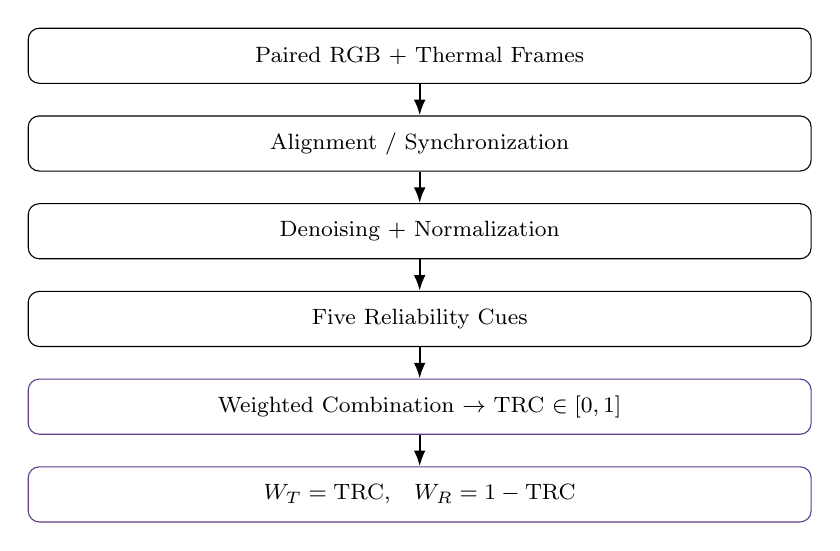
\begin{tikzpicture}[
box/.style={draw,rounded corners,align=center,minimum width=0.82\columnwidth,minimum height=7mm,font=\footnotesize},
arr/.style={-{Latex[length=2mm]},thick}
]
\node[box] (a) {Paired RGB + Thermal Frames};
\node[box,below=4mm of a] (b) {Alignment / Synchronization};
\node[box,below=4mm of b] (c) {Denoising + Normalization};
\node[box,below=4mm of c] (d) {Five Reliability Cues};
\node[box,below=4mm of d,draw=trcPurple] (e) {Weighted Combination $\rightarrow$ TRC $\in[0,1]$};
\node[box,below=4mm of e,draw=trcPurple] (f) {$W_T=\mathrm{TRC}$,\quad $W_R=1-\mathrm{TRC}$};
\foreach \x/\y in {a/b,b/c,c/d,d/e,e/f}
\draw[arr] (\x) -- (\y);
\end{tikzpicture}
\caption{TRC computation and reliability-to-fusion mapping.}
\label{fig:trcflow}
\end{figure}

% ============================================================
% VI. IMPLEMENTATION
% ============================================================

\section{Implementation and Experimental Setup}

\subsection{Development Stack}

The supplied implementation documentation identifies Python and C++ as programming languages, PyTorch and Ultralytics YOLO as the deep-learning stack, OpenCV and NumPy for computer vision, Matplotlib/Plotly for visualization, and CUDA-enabled NVIDIA GPU acceleration for deployment-oriented experiments. The broader planned stack includes Albumentations, Pillow, scikit-image, TorchMetrics, COCO tools, TensorBoard, and optional FastAPI/Uvicorn and ONNX Runtime components.

\begin{table}[!t]
\centering
\caption{TriNetra implementation stack}
\label{tab:stack}
\footnotesize
\begin{tabular}{p{0.25\columnwidth}p{0.64\columnwidth}}
\toprule
\textbf{Layer} & \textbf{Tools / Components}\\
\midrule
Programming & Python, C++\\
Deep learning & PyTorch; Ultralytics YOLOv8/YOLO family\\
Computer vision & OpenCV, NumPy, Pillow, scikit-image\\
Augmentation & Albumentations / synchronized RGB-T transforms\\
Data format & COCO conversion and paired RGB-T DataLoader\\
Reliability & Entropy, Laplacian variance, clipping, NMI, reprojection error\\
Tracking & ByteTrack / DeepSORT-type modular tracker\\
Visualization & Matplotlib, Plotly, TensorBoard\\
Deployment & NVIDIA CUDA GPU; planned API and ONNX Runtime path\\
Development & VS Code, Git, GitHub; configuration-driven YAML pipeline\\
\bottomrule
\end{tabular}
\end{table}

\subsection{Dataset and Data Preparation}

LLVIP is the principal paired visible-thermal dataset in the current implementation. The supplied project documentation describes Phase 2 as complete, including paired RGB-T loading, COCO conversion, and synchronized augmentation. FLIR thermal data and additional RGB-T benchmark data are identified as supplementary evaluation sources.

\begin{table}[!t]
\centering
\caption{Datasets identified for TriNetra evaluation}
\label{tab:datasets}
\footnotesize
\begin{tabular}{p{0.22\columnwidth}p{0.68\columnwidth}}
\toprule
\textbf{Dataset} & \textbf{Role in TriNetra}\\
\midrule
LLVIP & Primary paired RGB-T low-light surveillance dataset; current TRC pipeline verified end-to-end on LLVIP.\\
FLIR & Supplementary thermal/RGB-T evaluation source for robustness and generalization experiments.\\
Additional RGB-T benchmarks & Optional cross-dataset validation under varied day/night and degradation conditions.\\
\bottomrule
\end{tabular}
\end{table}

\subsection{Augmentation}

RGB and thermal images must undergo synchronized geometric transformations so that corresponding pixels remain spatially meaningful. The augmentation pipeline should preserve pair identity and apply equivalent geometric transforms to both modalities. Photometric transformations should be modality-aware because visible intensity and thermal intensity have different physical meanings.

\subsection{Detection Configuration}

The research plan specifies a YOLOv8-based detector with two modality streams exposing multi-scale features at P3/P4/P5. The visible branch can be initialized from pretrained weights, while the thermal branch and fusion blocks are trained using transfer learning. The recommended strategy is to initially freeze the pretrained visible backbone/neck/head, train the newly introduced thermal and fusion components, and optionally perform low-learning-rate fine-tuning.

A preliminary Stage-1 training run has since been completed with the
following resolved settings: a YOLOv8m \cite{yolov8} backbone at
$640\times512$ input resolution, AdamW optimizer with a cosine learning-rate
schedule (peak $1\times10^{-3}$), weight decay $5\times10^{-4}$,
confidence threshold 0.25 and IoU threshold 0.45 for NMS decoding.
The run used a batch size of 4 rather than the configured default of
16, which was found to exhaust available memory on the CPU-only
evaluation machine, and completed 4 of the planned 20 Stage-1 epochs
over 300 of the 9{,}903 available training images, with model
selection by mAP@0.50 on a disjoint 80-image held-out slice of the
validation split. Full results appear in
Section~\ref{sec:results}.

% ============================================================
% VII. EXPERIMENTAL DESIGN
% ============================================================

\section{Experimental Design}

The experimental design is organized to isolate the effect of reliability-aware fusion.

\subsection{Baseline Comparisons}

The following models should be evaluated under identical data splits and training/evaluation conditions:

\begin{table}[!t]
\centering
\caption{Required ablation and baseline experiments}
\label{tab:ablations}
\footnotesize
\begin{tabular}{p{0.18\columnwidth}p{0.70\columnwidth}}
\toprule
\textbf{ID} & \textbf{Configuration}\\
\midrule
B1 & RGB-only YOLO detector\\
B2 & Thermal-only YOLO detector\\
B3 & Conventional RGB-T fusion with fixed/equal weighting\\
B4 & TRC-gated RGB-T fusion (TriNetra-v1)\\
B5 & TRC + learned adaptive weighting using a small MLP (TriNetra-v2, optional research extension)\\
\bottomrule
\end{tabular}
\end{table}

This design follows the implementation strategy documented for TriNetra: establish a fixed-weight baseline first, then replace the fixed weighting mechanism with a learned MLP so that the effect of adaptive weighting can be isolated.

\subsection{Evaluation Metrics}

Detection performance should be reported using:

\begin{equation}
\mathrm{Precision}=\frac{TP}{TP+FP},
\end{equation}

\begin{equation}
\mathrm{Recall}=\frac{TP}{TP+FN},
\end{equation}

and

\begin{equation}
F_1=\frac{2PR}{P+R}.
\end{equation}

Mean average precision should be reported at IoU $=0.50$ and, where supported by the evaluation framework, across IoU thresholds from 0.50 to 0.95. Runtime should be measured using frames per second (FPS) and end-to-end latency. The same hardware and measurement procedure must be used across baselines.

\subsection{Reliability Stress Testing}

The TRC module should be evaluated independently of detector performance. The current stress-test conditions are:

\begin{enumerate}
    \item clean thermal input;
    \item blurred thermal input;
    \item saturated/clipped thermal input;
    \item flat or low-contrast thermal input;
    \item controlled RGB--thermal alignment perturbation.
\end{enumerate}

The objective is to test whether TRC changes monotonically or consistently in the expected direction as thermal information becomes less reliable.

% ============================================================
% VIII. RESULTS
% ============================================================

\section{Results}
\label{sec:results}

\subsection{TRC Distribution on Validation Data}
\label{sec:trcvalidation}

The current validation output contains 80 frames. The mean thermal reliability confidence is 0.758 and no frame falls below the configured 0.30 flagging threshold.

\begin{figure}[!t]
\centering
\fbox{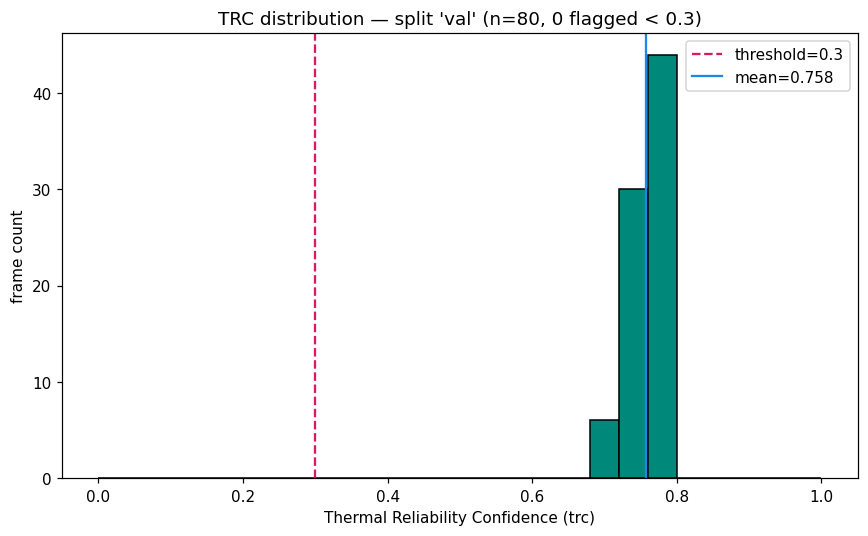
\includegraphics[width=0.96\columnwidth]{trc_report_val.png}}
\caption{TRC distribution over the validation split. The supplied evaluation output reports $n=80$, mean TRC $=0.758$, and zero frames below the 0.30 threshold.}
\label{fig:trcdistribution}
\end{figure}

The concentration of scores around the higher-reliability region indicates that the current validation subset is generally assigned a usable thermal confidence. This observation should not be interpreted as proof of detection improvement; it validates only the empirical distribution of the reliability estimator.

\subsection{TRC Under Synthetic Thermal Degradation}

The controlled stress test produces:

\begin{table}[!t]
\centering
\caption{Observed TRC under thermal degradation}
\label{tab:stress}
\footnotesize
\begin{tabular}{lc}
\toprule
\textbf{Condition} & \textbf{TRC}\\
\midrule
Clean & 0.67\\
Blur & 0.62\\
Saturation & 0.38\\
Flat / low-contrast & 0.40\\
\bottomrule
\end{tabular}
\end{table}

\begin{figure}[!t]
\centering
\fbox{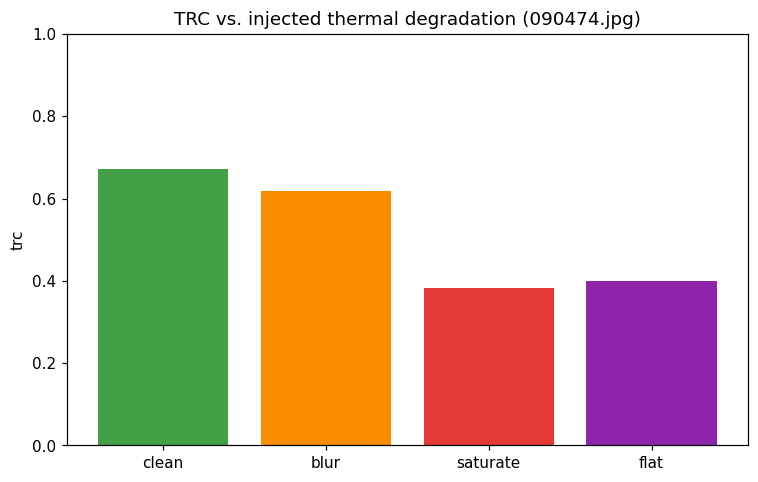
\includegraphics[width=0.96\columnwidth]{trc_stress_val.png}}
\caption{TRC response under the supplied thermal degradation stress test.}
\label{fig:trcstress}
\end{figure}

The results show a substantial reduction in TRC for saturation and flat thermal responses relative to the clean condition. Blur also produces a decrease, although the reduction is smaller. This supports the intended interpretation that the reliability score is sensitive to the tested degradation modes.

\subsection{Per-Frame TRC Component Examples}

Two supplied preprocessing reports provide frame-level examples. For frame 030396.jpg, the reported TRC is 0.615 with component values of contrast 0.92, gradient 0.11, saturation 0.99, mutual information 0.05, and alignment error reported as 1.00. For frame 091028.jpg, the corresponding TRC is 0.640 with contrast 0.95, gradient 0.20, saturation 0.98, mutual information 0.07, and alignment error reported as 1.00.

\begin{figure}[!t]
\centering
\begin{subfigure}{0.48\columnwidth}
\centering
\fbox{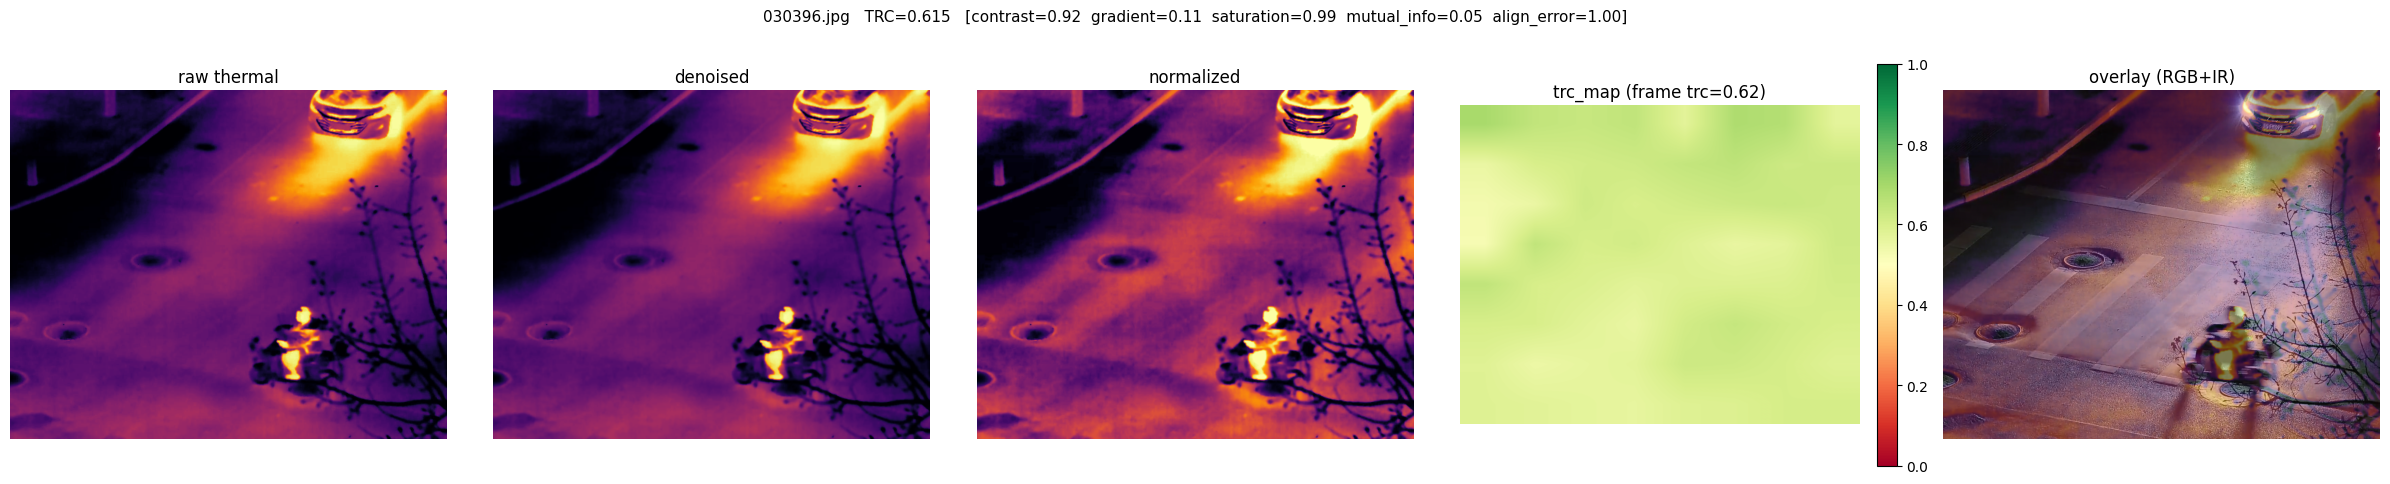
\includegraphics[width=\linewidth]{preproc_val_030396.png}}
\caption{030396.jpg}
\end{subfigure}
\hfill
\begin{subfigure}{0.48\columnwidth}
\centering
\fbox{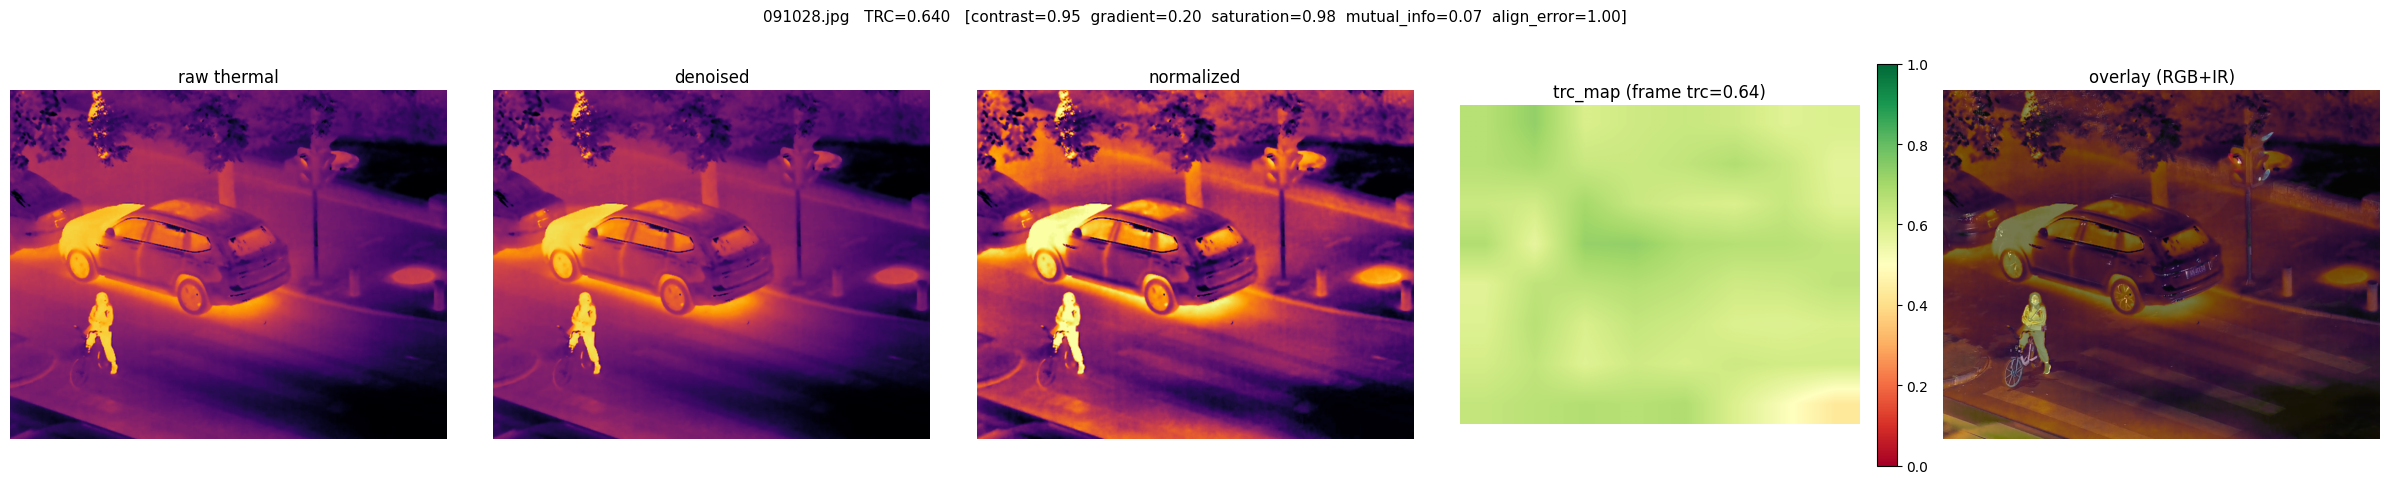
\includegraphics[width=\linewidth]{preproc_val_091028.png}}
\caption{091028.jpg}
\end{subfigure}
\caption{Representative thermal preprocessing and TRC-map outputs.}
\label{fig:preprocessing}
\end{figure}

The repeated alignment-error value of 1.00 requires verification before a final journal/conference version is submitted. In particular, the implementation should confirm whether this quantity denotes normalized error, normalized quality, or a metric that has saturated at its upper bound. The paper should use the exact implementation convention.

\subsection{Qualitative RGB-T Observations}

The supplied paired visualizations show complementary information across RGB and thermal modalities. In low-light scenes, RGB retains scene texture and contextual structure while thermal emphasizes warm objects and pedestrians. The overlay visualizations illustrate the potential value of combining the two streams.

\begin{figure*}[!t]
\centering
\begin{subfigure}{0.31\textwidth}
\centering
\fbox{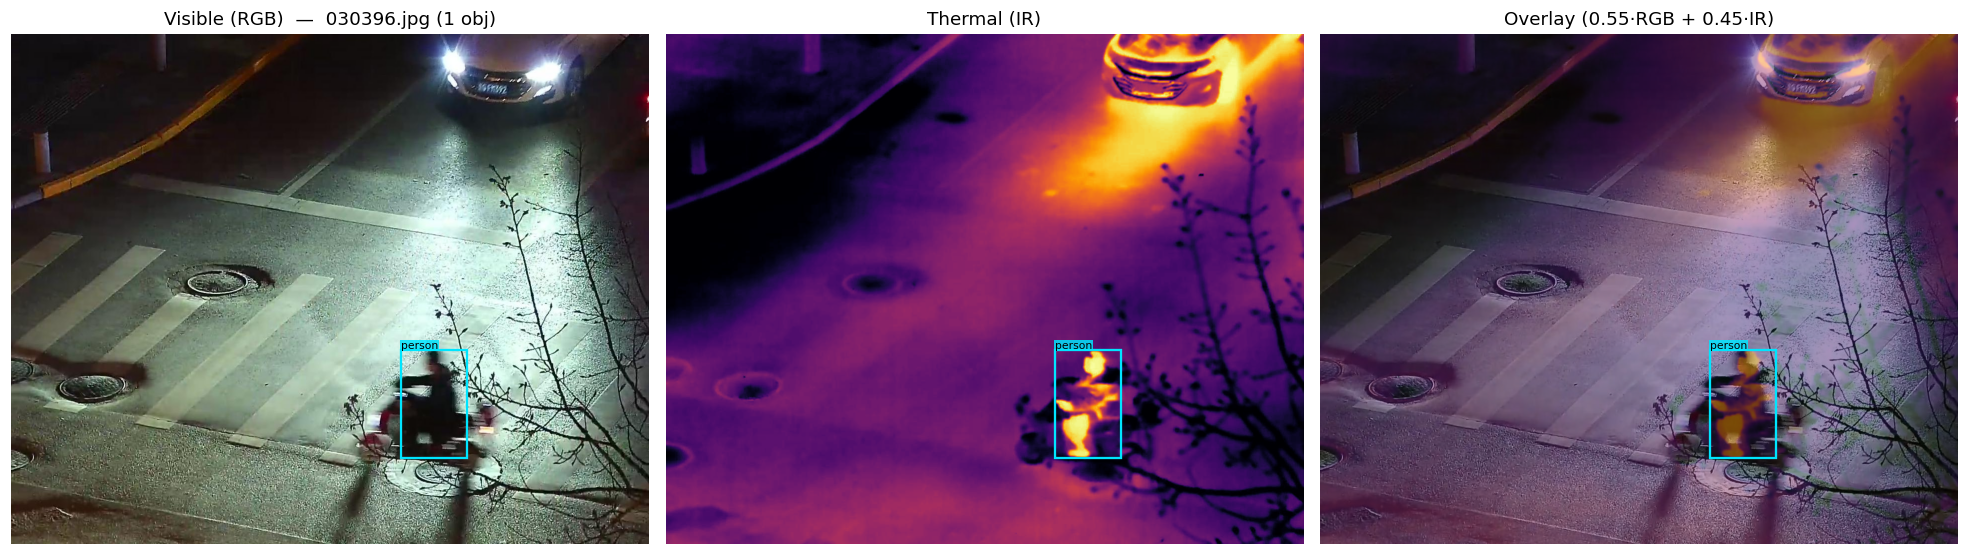
\includegraphics[width=\linewidth]{val_030396_pair.png}}
\caption{030396.jpg}
\end{subfigure}
\hfill
\begin{subfigure}{0.31\textwidth}
\centering
\fbox{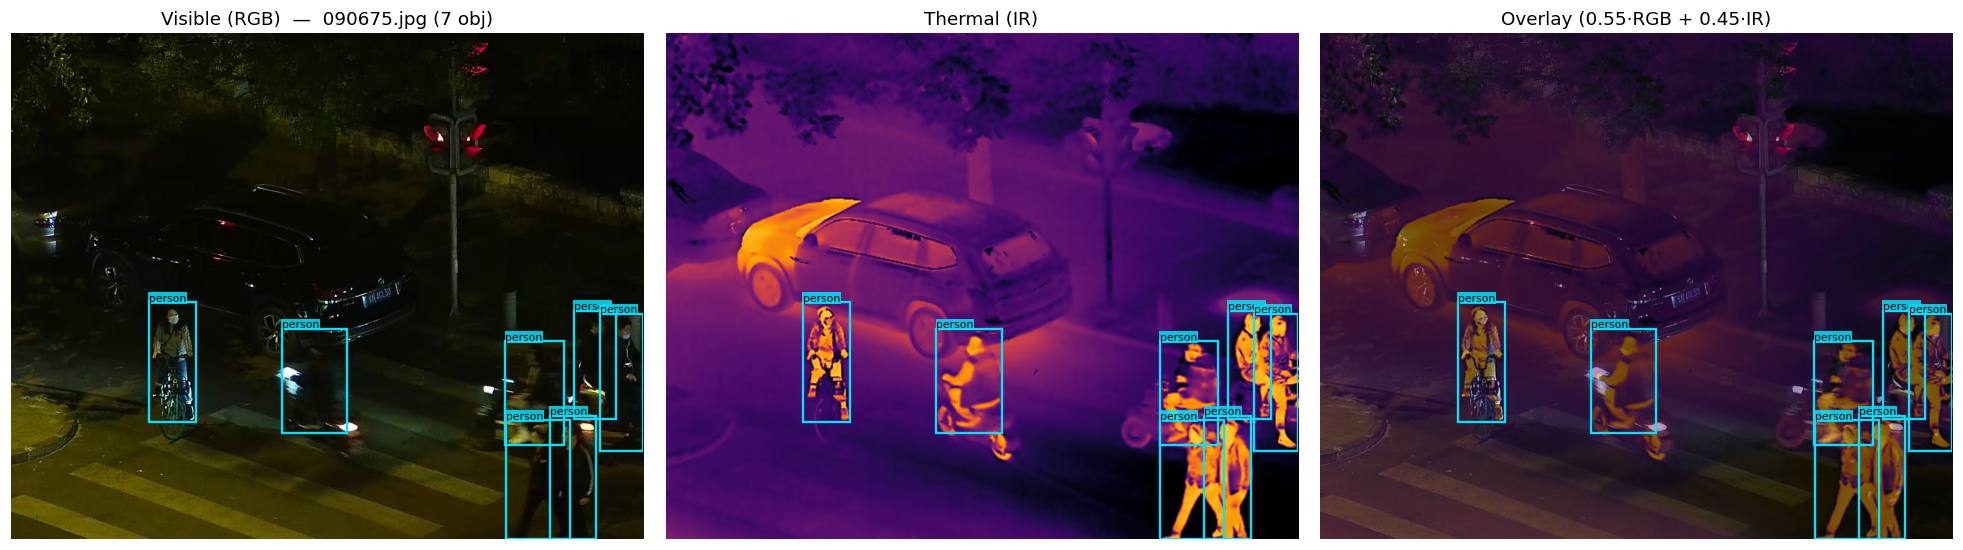
\includegraphics[width=\linewidth]{val_090675_pair.png}}
\caption{090675.jpg}
\end{subfigure}
\hfill
\begin{subfigure}{0.31\textwidth}
\centering
\fbox{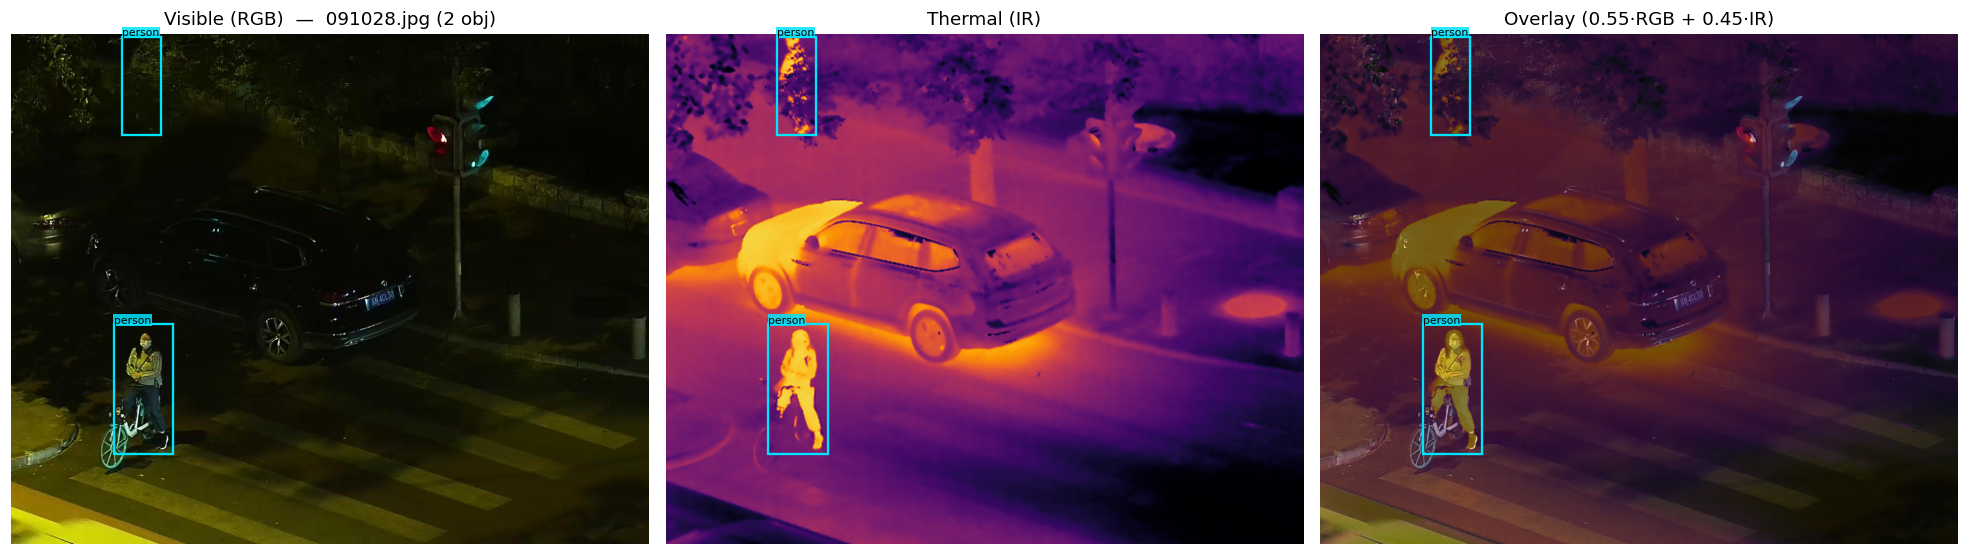
\includegraphics[width=\linewidth]{val_091028_pair.png}}
\caption{091028.jpg}
\end{subfigure}
\caption{Representative RGB-T paired observations and detections from the validation examples supplied with the current implementation.}
\label{fig:qualitative}
\end{figure*}

\subsection{Detection Performance}

A preliminary TriNetra-v1 (TRC-gated fusion) checkpoint has been
trained and evaluated end-to-end; the single-modality, fixed-fusion,
and learned-weight variants required to complete the comparative
table have not yet been run under the identical protocol, so those
rows remain placeholders.

\textbf{Training run.} Stage 1 (visible backbone, neck, and head
frozen; thermal backbone and fusion blocks trainable) was run for 4
epochs on 300 images sampled from the 9{,}903-image train pool, with
model selection against a disjoint 80-image held-out slice of the
validation split never used for training. Training loss fell
monotonically across all four epochs (box/cls/DFL: 1.602/0.796/1.419
$\rightarrow$ 1.395/0.565/1.278). Validation mAP@0.50 showed a
transient near-zero reading after epoch 1 (0.0001) before recovering
to 0.879 at epoch 2 and reaching 0.893 at epoch 4 --- consistent with
early instability while the newly initialized thermal branch and
fusion gate adjust, rather than a persistent failure.

\textbf{Full test-set evaluation.} The 80-image validation figure
above is a small sample and may not be representative. The resulting
checkpoint was therefore also evaluated on the complete, official
LLVIP test split --- all 3{,}463 images, none seen during training or
model selection --- giving the statistically stable result in
Table~\ref{tab:mainresults}: mAP@0.50\,=\,0.770, mAP@0.50:0.95\,=\,0.472,
AP@0.75\,=\,0.519, and AR@10/AR@100\,=\,0.527, over 9{,}729 detections.
Every one of the 3{,}463 test images fell in the TRC ``clean'' bin
(mean TRC 0.765), matching the earlier validation-split observation
(Section~\ref{sec:trcvalidation}) that real LLVIP frames rarely
register as thermally degraded.

\begin{table*}[!t]
\centering
\caption{End-to-end detection comparison on the full LLVIP test split (3{,}463 images). Baseline and TriNetra-v2 rows remain placeholders pending training under an identical protocol; ``--'' marks metrics not yet measured for TriNetra-v1.}
\label{tab:mainresults}
\footnotesize
\begin{tabular}{lccccccl}
\toprule
\textbf{Method} & \textbf{Precision} & \textbf{Recall} & \textbf{AR@100} & \textbf{mAP@50} & \textbf{mAP@50:95} & \textbf{FPS} & \textbf{Notes}\\
\midrule
RGB-only & -- & -- & -- & -- & -- & -- & Baseline (not yet run)\\
Thermal-only & -- & -- & -- & -- & -- & -- & Baseline (not yet run)\\
Fixed RGB-T & -- & -- & -- & -- & -- & -- & Fixed weighting (not yet run)\\
TriNetra-v1 & -- & -- & 0.527 & 0.770 & 0.472 & -- & TRC-gated fusion; 300/9{,}903 train images, 4/20 epochs, CPU\\
TriNetra-v2 & -- & -- & -- & -- & -- & -- & TRC + MLP weights (not yet run)\\
\bottomrule
\end{tabular}
\end{table*}

\textbf{Context from the literature.} No numerical superiority claim
can be made until the baseline rows above are measured under the same
protocol. For scale, prior work reports substantially higher mAP@50
on LLVIP when trained at full scale: single-modality YOLOv5 baselines
of 90.8 (RGB) and 94.6 (thermal), and fused results up to 97.7--98.1
with dedicated fusion architectures \cite{eef}, all trained for many
more epochs over the complete training set. The gap between those
figures and the 0.770 measured here is expected given that TriNetra-v1
was trained on roughly 3\% of the available training images for 4 of
a planned 20 epochs on CPU, and should not be read as a statement
about the TRC-gating mechanism itself; closing that gap under a
matched training budget is the immediate next experiment.

% ============================================================
% IX. ABLATION
% ============================================================

\section{Ablation and Sensitivity Analysis}

\subsection{Five-Cue TRC Ablation}

To establish that the TRC is not dominated by a single cue, each component should be removed individually while all remaining conditions are kept constant.

\begin{table}[!t]
\centering
\caption{TRC cue ablation template}
\label{tab:trcablation}
\scriptsize
\begin{tabular}{lcccccc}
\toprule
\textbf{Configuration} & $S_C$ & $S_G$ & $S_S$ & $S_{MI}$ & $S_A$ & \textbf{TRC}\\
\midrule
All five cues & \checkmark & \checkmark & \checkmark & \checkmark & \checkmark & --\\
No contrast & -- & \checkmark & \checkmark & \checkmark & \checkmark & --\\
No gradient & \checkmark & -- & \checkmark & \checkmark & \checkmark & --\\
No saturation & \checkmark & \checkmark & -- & \checkmark & \checkmark & --\\
No mutual information & \checkmark & \checkmark & \checkmark & -- & \checkmark & --\\
No alignment & \checkmark & \checkmark & \checkmark & \checkmark & -- & --\\
\bottomrule
\end{tabular}
\end{table}

\subsection{Degradation-Severity Sensitivity}

For each degradation type, multiple severity levels should be generated. Let $\delta$ denote degradation severity. A useful diagnostic is:

\begin{equation}
\rho_{\mathrm{TRC}}=
\operatorname{corr}(\mathrm{TRC},-\delta),
\end{equation}

where a positive correlation indicates that TRC decreases as degradation increases when the sign convention is defined accordingly. The final paper should report the correlation coefficient and confidence interval only after repeated experiments.

\subsection{Fusion-Weight Sensitivity}

Because $W_T=\mathrm{TRC}$ and $W_R=1-\mathrm{TRC}$, the effective thermal contribution should be inspected across the validation distribution. A histogram of $W_T$ is equivalent to the TRC distribution under the current mapping. This provides an interpretable link between reliability estimation and fusion behaviour.

% ============================================================
% X. THREAT INTELLIGENCE
% ============================================================

\section{Surveillance and Threat-Intelligence Layer}

TriNetra is intended to extend beyond object detection toward surveillance-oriented temporal reasoning. The architecture includes multi-object tracking, behaviour analysis, contextual threat assessment, and explainable alert generation. These components are modular and should not be conflated with the current TRC validation results.

\subsection{Tracking}

The detector produces object bounding boxes and confidence scores. A multi-object tracker associates detections across consecutive frames and maintains persistent object identities. Candidate tracking outputs include object IDs, trajectories, dwell time, motion direction, and estimated speed.

\subsection{Behaviour Analysis}

Behaviour analysis can use temporal features such as:

\begin{equation}
v_t=\frac{\|\mathbf{p}_t-\mathbf{p}_{t-\Delta t}\|}{\Delta t},
\end{equation}

where $\mathbf{p}_t$ is the object centroid at time $t$. Directional change, dwell time, and trajectory deviation can be combined with spatial context.

\subsection{Contextual Threat Score}

The copyright-level design describes hierarchical threat reasoning using contextual cues such as zone violation, abnormal movement, density/congestion, and risk factors. A generic formulation is:

\begin{equation}
T=
\alpha Z+
\beta B+
\gamma M+
\delta D+
\eta C,
\label{eq:threat}
\end{equation}

where $Z$ is zone violation, $B$ behaviour abnormality, $M$ motion-pattern evidence, $D$ density/congestion, and $C$ contextual confidence. The coefficients should be calibrated empirically and must not be presented as validated values unless measured.

\subsection{Explainability}

For each alert, the system is intended to expose the principal evidence that contributed to the decision, such as:

\begin{itemize}
    \item detected object and class;
    \item object ID and trajectory;
    \item RGB and thermal reliability;
    \item contextual event;
    \item threat score;
    \item final threat level;
    \item timestamp and location/zone identifier.
\end{itemize}

This design provides a human-readable chain from sensing to alert rather than producing an unexplained binary output.

% ============================================================
% XI. COMPARISON
% ============================================================

\section{Comparison With Related RGB-T Strategies}

\begin{table*}[!t]
\centering
\caption{Conceptual comparison of TriNetra with supplied related RGB-T approaches}
\label{tab:relatedcomparison}
\footnotesize
\begin{tabular}{p{0.18\textwidth}p{0.15\textwidth}p{0.15\textwidth}p{0.15\textwidth}p{0.15\textwidth}p{0.14\textwidth}}
\toprule
\textbf{Criterion} & \textbf{TFDet} & \textbf{QDFM} & \textbf{DENet} & \textbf{GEM-YOLO} & \textbf{TriNetra}\\
\midrule
Primary focus & Target-aware fusion/refinement & Quality-aware decision fusion & Failure-aware feature reconstruction & Lightweight gated fusion & Reliability-aware surveillance pipeline\\
Reliability signal & Learned feature relationships & Evidential uncertainty & Illumination/similarity-aware weighting & Learned multimodal gate & Explicit five-cue TRC\\
Fusion stage & Feature fusion & Decision fusion & Feature processing/fusion & Feature fusion & Pre-fusion reliability gating + feature fusion\\
Modality failure & Indirectly handled through feature refinement & Explicitly targeted & Explicitly targeted & Adaptive gating & Explicit stress-tested reliability score\\
Interpretability of reliability & Limited & Evidence-based & Learned & Learned gate & High; individual cues exposed\\
Detector dependence & Detection-oriented & Detection-oriented & Detection-oriented & YOLO-oriented & Designed as detector-agnostic module\\
Tracking/threat layer & No central focus & No central focus & No central focus & No central focus & Included in system architecture\\
Real-time orientation & Reported competitive efficiency & Not primary contribution & Not primary contribution & Strong emphasis & Deployment-oriented design\\
\bottomrule
\end{tabular}
\end{table*}

This comparison is conceptual and describes the architectural emphasis of each approach; it is not a claim that the methods use identical datasets, detector backbones, or experimental protocols.

% ============================================================
% XII. DISCUSSION
% ============================================================

\section{Discussion}

\subsection{Interpretation of Current Findings}

The current results provide preliminary evidence relevant to H2: whether an interpretable thermal reliability score can be computed consistently over paired RGB-T observations and whether it responds to controlled thermal degradation. The validation distribution demonstrates that the score is numerically stable within the tested subset, while the stress test demonstrates lower values for several degradation modes.

The stress-test result is particularly important because it is independent of detector training. It tests the reliability estimator itself. However, a detector-level conclusion requires the next experiment: the same degraded inputs must be evaluated using RGB-only, thermal-only, fixed-fusion, and TRC-gated models. Only then can a relationship between reliability-aware fusion and detection performance be established.

A separate, complementary finding now exists on the detector side. Training TriNetra-v1 end-to-end on real data shows that the architecture is trainable with a stable and coherent loss curve, and that it reaches a plausible full-test-set mAP given its minimal training budget. The transient near-zero validation mAP observed immediately after epoch 1 (Section~\ref{sec:results}) is worth flagging as an open question rather than dismissing: it may reflect the newly initialized thermal branch and fusion gate temporarily overwhelming the otherwise-strong frozen-backbone prior before the fusion weights settle, but distinguishing that explanation from an optimizer or learning-rate sensitivity specific to very small batches would require repeating the run with different seeds and learning rates. Neither this detector result nor the TRC stress test, individually, tests H1; only the completed baseline suite in Table~\ref{tab:mainresults}, trained under a matched protocol, can do that.

\subsection{Interpretability}

A principal advantage of the current formulation is that a TRC value can be decomposed into its five constituent cues. This allows an engineer to inspect whether a low score is caused by poor contrast, weak edge information, excessive clipping, low cross-modal agreement, or poor alignment. This is more transparent than a learned fusion gate whose internal weighting is not directly interpretable.

\subsection{Limitations}

Several limitations must be addressed in the final version.

First, the current TRC implementation is frame-level rather than fully spatial. A single score can suppress or enhance the thermal stream globally even when reliability varies strongly within a frame. A spatial TRC map is therefore a natural extension.

Second, the five cues are hand-designed. Their relative weights may not be optimal across datasets, sensors, or environments. The planned MLP-based adaptive weighting experiment provides a way to investigate learned weighting while preserving the same experimental pipeline.

Third, mutual information and alignment measures can be sensitive to preprocessing and registration. The repeated alignment-related value reported as 1.00 in the supplied per-frame outputs must be inspected before publication.

Fourth, the current paper distinguishes the verified TRC stage from the planned end-to-end detection and threat modules. The latter require controlled experiments before quantitative claims can be made.

Finally, synthetic degradation does not perfectly reproduce real sensor failure. Future evaluation should include naturally occurring adverse conditions and, where possible, real sensor interference.

Sixth, the TriNetra-v1 detection result reported in Section~\ref{sec:results} is preliminary: it was trained on roughly 3\% of the available training images for 4 of a planned 20 Stage-1 epochs on CPU hardware, without the single-modality or fixed-fusion baselines needed to test H1 comparatively, and without precision, recall, F1, or FPS measurement. It should be read as evidence that the architecture trains and generalizes correctly, not as a performance claim relative to prior RGB-T detectors or to the fixed-fusion/single-modality baselines this paper defines.

% ============================================================
% XIII. FUTURE WORK
% ============================================================

\section{Future Work}

The TRC-gated YOLOv8 fusion implementation now trains end-to-end
(Section~\ref{sec:results}); the immediate research objective is to
scale that training to GPU hardware and complete the full Stage-1
schedule (20 epochs over all 9{,}903 training images, rather than the
4-epoch, 300-image preliminary run reported here), then train the
RGB-only, thermal-only, and fixed-weight RGB-T baselines under the
identical protocol so Table~\ref{tab:mainresults} can be completed
and H1 tested comparatively. The next stage after that is the learned
weighting variant in which a small MLP receives the five quality cues
and predicts adaptive modality weights. This provides a clean
comparison between interpretable fixed weighting and learned adaptive
weighting.

A second direction is region-adaptive reliability. Instead of a scalar TRC, the system can estimate:

\begin{equation}
\mathbf{R}_T(x,y)\in[0,1],
\end{equation}

allowing different regions of a frame to contribute thermal information at different strengths.

Cross-modal attention and lightweight edge deployment are additional directions identified in the project documentation. Wider benchmarking across LLVIP, FLIR, and other RGB-T datasets is also necessary to determine whether the reliability formulation generalizes beyond the current validation subset.

The threat-intelligence layer can subsequently be evaluated using tracking metrics, event-detection precision/recall, alert latency, and false-alarm rate. Such evaluation should be conducted separately from object-detection metrics.

% ============================================================
% XIV. CONCLUSION
% ============================================================

\section{Conclusion}

This paper presented TriNetra, a reliability-aware RGB-T surveillance framework centred on the TriNetra Reliability Coefficient. The approach explicitly estimates thermal reliability from five normalized cues---contrast, gradient strength, saturation, cross-modal mutual information, and alignment quality---and maps the resulting score to complementary modality weights for adaptive fusion.

The current implementation provides an end-to-end TRC preprocessing and evaluation pipeline. On the supplied validation output, 80 frames produced a mean TRC of 0.758 with no frame below the 0.30 flagging threshold. In a controlled degradation test, TRC decreased from 0.67 for clean thermal input to 0.62 under blur, 0.38 under saturation, and 0.40 for flat/low-contrast input. These findings support the intended sensitivity of the reliability estimator to the tested thermal degradation modes.

A preliminary TRC-gated fusion detector (TriNetra-v1) has since been
trained and evaluated end-to-end on the complete, official LLVIP test
split, reaching mAP@0.50\,=\,0.770 and mAP@0.50:0.95\,=\,0.472 after
only 4 of a planned 20 Stage-1 epochs on roughly 3\% of the available
training images. This demonstrates that the architecture trains
stably and generalizes to genuinely held-out data, but it is not yet
a test of H1: the central remaining experimental question is still
whether this reliability signal improves object detection compared
with single-modality and fixed-fusion baselines trained under the
same protocol. The paper therefore defines a controlled YOLOv8
evaluation and ablation protocol, including RGB-only, thermal-only,
fixed RGB-T, TRC-gated fusion, and optional learned-weight variants.
Once those baseline experiments are completed at matching scale, the
remaining placeholder rows in Table~\ref{tab:mainresults} can be
replaced with measured values and statistical analysis.

TriNetra is consequently positioned as a modular bridge between low-level multimodal quality assessment and higher-level surveillance intelligence. Its reliability signal is intended to provide a transparent control mechanism for multimodal fusion while allowing the detector, tracker, and downstream reasoning components to remain modular.

% ============================================================
% APPENDIX: FIGURE/RESULT CHECKLIST
% ============================================================



% ============================================================
% REFERENCES
% ============================================================

\begin{thebibliography}{00}

\bibitem{songSurvey}
K. Song, Y. Zhao, L. Huang, Y. Yan, and Q. Meng,
``RGB-T image analysis technology and application: A survey,''
\emph{Engineering Applications of Artificial Intelligence},
vol. 120, Art. no. 105919, 2023,
doi: 10.1016/j.engappai.2023.105919.

\bibitem{tfdet}
X. Zhang, X. Zhang, J. Wang, J. Ying, Z. Sheng, H. Yu,
C. Li, and H.-L. Shen,
``TFDet: Target-Aware Fusion for RGB-T Pedestrian Detection,''
\emph{IEEE Transactions on Neural Networks and Learning Systems},
vol. 36, no. 7, 2025,
doi: 10.1109/TNNLS.2024.3443455.

\bibitem{qdfm}
H. Yu, R. Luo, X. Wang, D. Wang, Q. Li, and S. Qiao,
``Robust RGB-T Object Detection via Quality-Aware Decision Fusion
Based on Dempster--Shafer Theory,''
\emph{IEEE Sensors Journal},
vol. 25, no. 13, 2025.

\bibitem{denet}
Q. Wang, Y. Sun, Y. Chi, and T. Shen,
``RGB-T Object Detection With Failure Scenarios,''
\emph{IEEE Journal of Selected Topics in Applied Earth Observations
and Remote Sensing},
vol. 18, 2025,
doi: 10.1109/JSTARS.2024.3523408.

\bibitem{eef}
T. Hao, J. Yang, S. Zhang, and S. Wu,
``EEF: Energy score-guided feature enhancement fusion method for RGB
and thermal infrared images object detection,''
\emph{Signal Processing},
vol. 239, Art. no. 110231, 2026,
doi: 10.1016/j.sigpro.2025.110231.

\bibitem{gemyolo}
L. Wang, Z. Bao, and D. Lu,
``GEM-YOLO: A Lightweight and Real-Time RGBT Object Detector with
Gated Multimodal Fusion,''
\emph{Sensors},
vol. 26, no. 7, Art. no. 2035, 2026,
doi: 10.3390/s26072035.

\bibitem{deepFusion}
F. Zhao, C. Zhang, and B. Geng,
``Deep Multimodal Data Fusion,''
\emph{ACM Computing Surveys},
vol. 56, no. 9, Art. no. 216, 2024,
doi: 10.1145/3649447.

\bibitem{yolov8}
G. Jocher, A. Chaurasia, and J. Qiu,
``Ultralytics YOLOv8,''
version 8.4, 2023. [Online]. Available:
\url{https://github.com/ultralytics/ultralytics}.

\end{thebibliography}

\appendices

\section{Resolved Implementation Configuration}

The following parameters are fixed according to the current TriNetra
implementation and project configuration.

\begin{table}[!t]
\centering
\caption{Resolved TriNetra implementation parameters}
\label{tab:resolvedparams}
\footnotesize
\begin{tabular}{p{0.39\columnwidth}p{0.47\columnwidth}}
\toprule
\textbf{Parameter} & \textbf{Value} \\
\midrule
Dataset & LLVIP \\
Total RGB-T pairs & 15,488 \\
Total annotations & 42,432 \\
Train / Validation / Test & 9,903 / 2,122 / 3,463 \\
Native resolution & $1280\times1024$ \\
Model input resolution & $640\times512$ \\
RGB channels & 3 \\
Thermal channels & 1 \\
Detector & YOLOv8m \\
Pretrained weights & COCO pretrained \\
Ultralytics version & 8.4.89 \\
Fusion scales & P3 / P4 / P5 \\
Fusion strides & 8 / 16 / 32 \\
TRC cue weights & 0.2 each \\
Gradient normalization constant $K$ & 15 \\
TRC type & Scalar frame-level \\
Spatial TRC map & Implemented as optional extension \\
LLVIP alignment & Identity / pass-through \\
Alignment reprojection error & 0 for aligned LLVIP pairs \\
Validation frames & 80 \\
Mean TRC & 0.758 \\
TRC standard deviation & 0.024 \\
Minimum TRC & 0.694 \\
Maximum TRC & 0.787 \\
Frames below TRC 0.30 & 0 / 80 \\
\midrule
\multicolumn{2}{l}{\textit{Preliminary TriNetra-v1 training run}} \\
PoC train images (of 9{,}903) & 300 \\
PoC held-out val images (of 2{,}122) & 80 \\
PoC epochs (of 20 planned) & 4 \\
PoC batch size & 4 \\
PoC hardware & CPU only (no CUDA GPU) \\
Ultralytics version (PoC run) & 8.4.150 \\
Full test images evaluated & 3,463 \\
PoC mAP@0.50 (full test) & 0.770 \\
PoC mAP@0.50:0.95 (full test) & 0.472 \\
PoC mean TRC (full test) & 0.765 \\
\bottomrule
\end{tabular}
\end{table}

\section{Hypothesis-Stage Scope}

This manuscript is intentionally presented at the hypothesis and
prototype-validation stage. The measured TRC validation and thermal
degradation results are reported as preliminary evidence relevant to
H2. A first measured end-to-end detection result also now exists for
TriNetra-v1 (mAP@0.50\,=\,0.770, mAP@0.50:0.95\,=\,0.472 on the full
LLVIP test split; Section~\ref{sec:results}), obtained from a
4-epoch, 300-image preliminary training run on CPU hardware. The
principal H1 claim---improved end-to-end RGB-T object detection
through reliability-aware fusion \emph{relative to single-modality
and fixed-fusion baselines}---remains a testable hypothesis and is
not presented as a confirmed result, because those baselines have not
yet been trained under the identical protocol.

Precision, recall, F1, FPS, latency, tracking accuracy, and
threat-classification accuracy remain unmeasured and are not claimed
in this version.

\end{document}
